\documentclass[aps,floatfix,11pt]{revtex4-1}
\usepackage{bm}%bold math
\usepackage{graphicx}
\usepackage{amsmath}
\usepackage{amssymb}
\usepackage{setspace}
\linespread{1}

\begin{document}

\title{Notes}

\date{\today}

\begin{abstract}
    
\end{abstract}

\maketitle 

\section{Misc}
At the RK point the ground state is the short-range resonating valence bond state

\begin{equation}
    \label{}
    \left| \Psi_{RVB} \right\rangle = \sum_{C} \left| C \right\rangle
\end{equation}
    
\noindent
where $\{C\}$ is the set of fully packed dimer configurations.

\begin{equation}
    \label{}
    \| \Psi_{RVB} \|^2 = Z_{classical dimer}
\end{equation}

i.e. the norm of $\Psi_{RVB}$ is the partition function of the classical dimer model.
\\
all above is from Fradkin.
\\

$U(1)$ gauge theory describes low-energy strong local correlations.
Coupling a $U(1)$ gauge field to a charge $N$ matter field reduces the gauge symmetry to $Z_N$ gauge
field (for $N>1$). 

The structure of the quantum dimer models phase diagrams depends on if a lattice is bipartite or
not; if it is bipartite it also depends on the coordination number. Most of the time the valence
bond crystal is the ground state.

The Hamiltonian of the quantum dimer model is split in the resonance term and the diagonal term. The
resonance term being the kinetic energy term and the diagonal term being the potential energy term
diagonal term being the potential energy term.
\begin{equation}
    \label{}
    H = H_{res} + H_{diag}
\end{equation}



\section{Dimer Model}

\subsection{Correlation Functions}

Here we check the implementation of our numerical methods. First we validate that the dimer pair
correlations in a fully packed dimer model decay as $1/r^2$. Second we validate that the monomer
pair (defect) correlations in a fully packed dimer model decay as $1/r^{1/2}$ ($1/r^{1/3}$ in the
fully packed loop model). In fig. \ref{fig:dimer_dimer_cor} we show a histogram of the correlation
function 
\begin{equation}
    \label{}
    C_{dimer}(0,r) = \langle s_0 s_r \rangle -\langle s_0 \rangle \langle s_r \rangle
\end{equation}

\noindent
for a lattice size of $64\times 64$ The disconnected piece of the correlation function is

\begin{equation}
    \label{}
    \langle s_0 \rangle \langle s_r \rangle = \frac{1}{4}\frac{1}{4} = \frac{1}{16}.
\end{equation}

\noindent
The connected component is calculated numerically, in this case, $s_0$ is the value of the link at the
right of the $(0,0)$ vertex and $s_r$ are only chosen from the same vertical column of links.
In fig. \ref{fig:dimer_dimer_cor_log} we show a log log plot of the relevent half of the data
shown in fig. \ref{fig:dimer_dimer_cor}. Using a weighted fit of on points $[3,9]$, shown in fig.
\ref{fig:fit_dm_dm_64x64} we find the slope of the line to be $-2.4833\pm 0.0090$.

We now look at the same correlation function on a $128\times128$ lattice.
Using a weighted fit of on points $[3,13]$, shown in fig.
\ref{fig:fit_dm_dm_128x128} we find the slope of the line to be $-2.4203\pm 0.0106$.

Now the correlation function on a $256\times256$ lattice.
Using a weighted fit of on points $[3,14]$, shown in fig.
\ref{fig:fit_dm_dm_256x256} we find the slope of the line to be $2.3057\pm 0.0269$.


\begin{figure}[h]
    \centering
    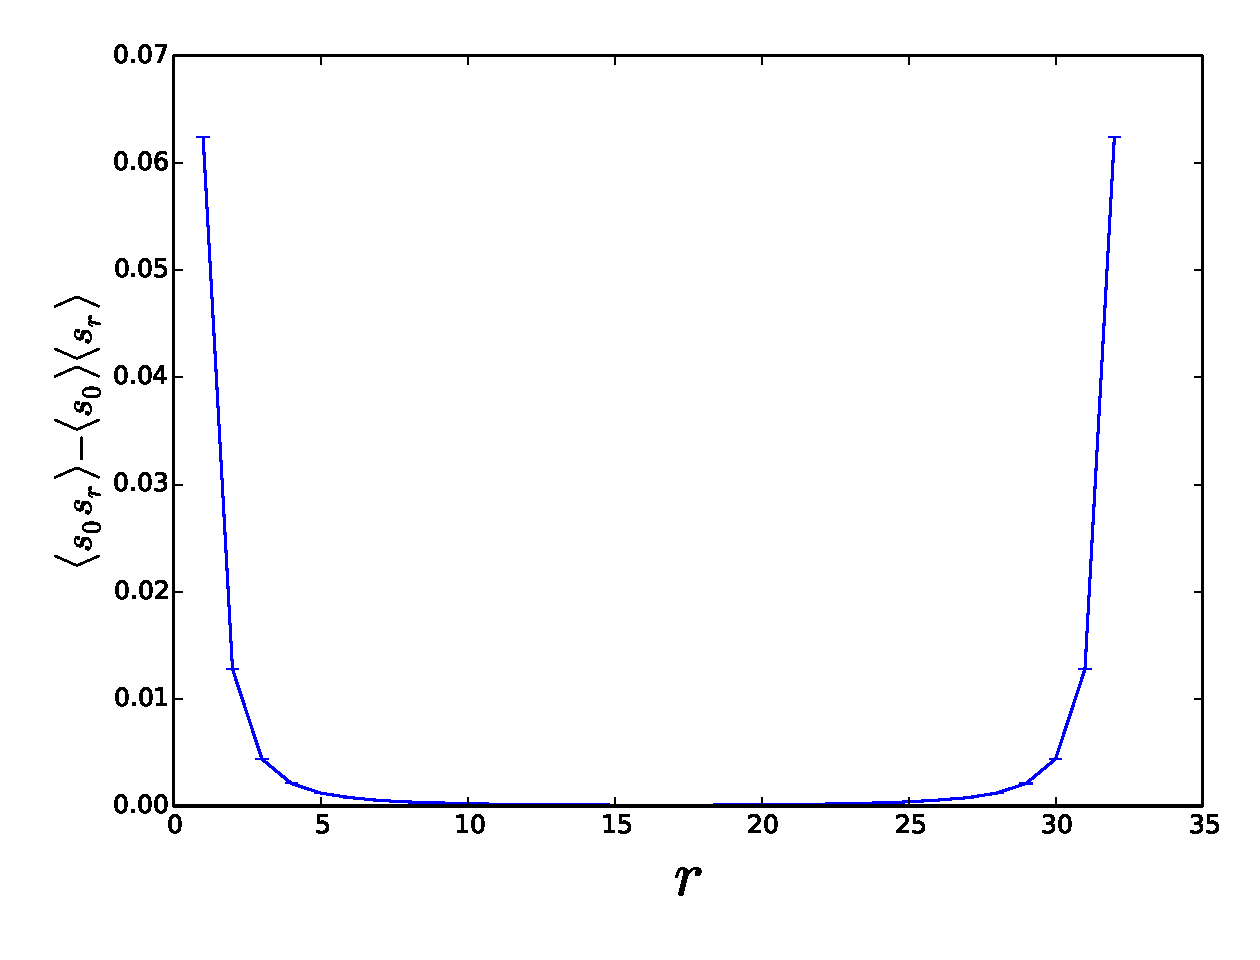
\includegraphics[width=8.5 cm]{dimer_dimer_cor}
    \caption{lattice size: $64\times64$. Number of bins: 80,000. Each bin averaged over 50,000
    configurations. Each configuration used was spaced by 4 random walks.\label{fig:dimer_dimer_cor}}
\end{figure}

\begin{figure}[h]
    \centering
    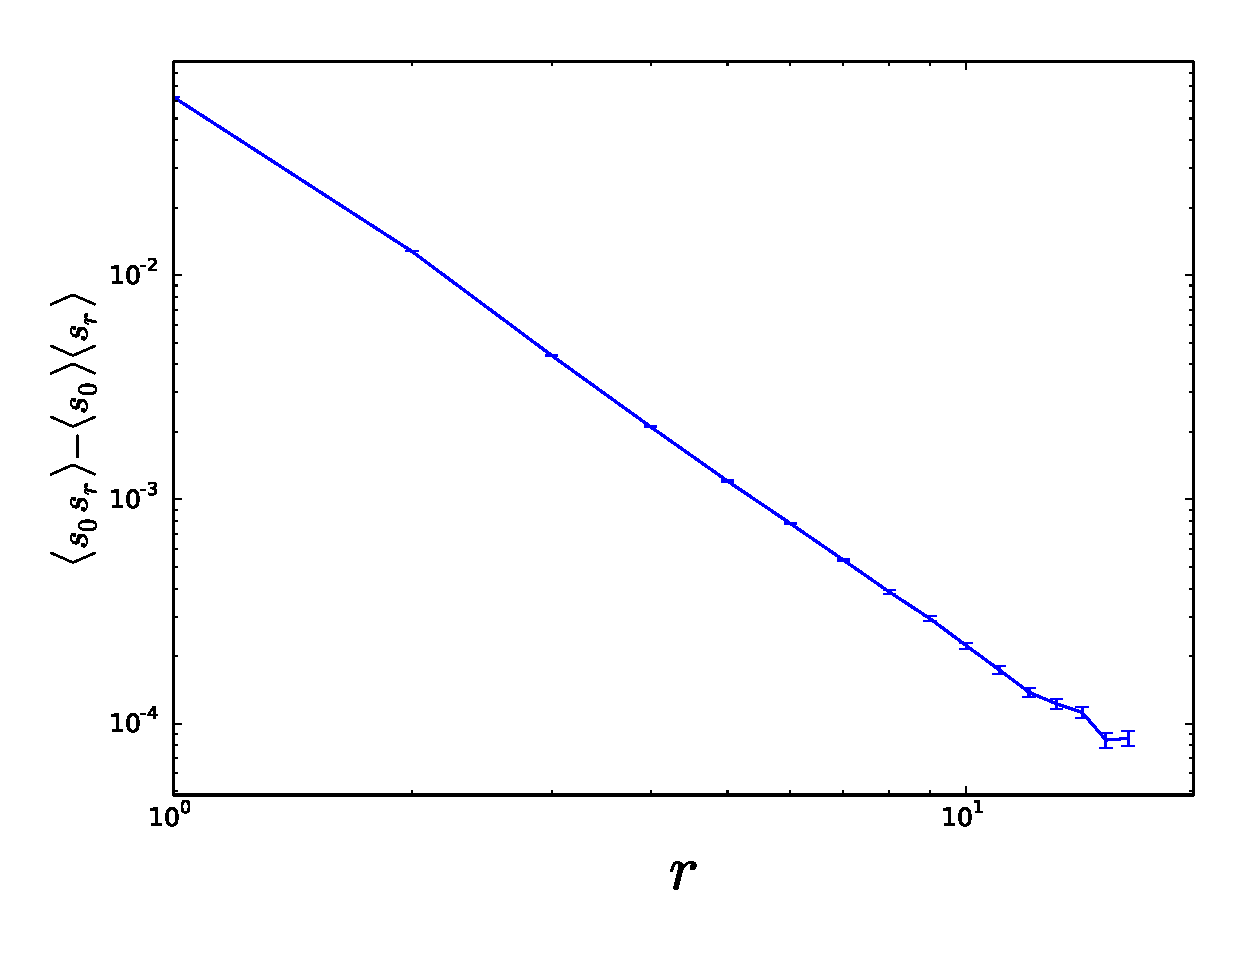
\includegraphics[width=8.5 cm]{dimer_dimer_cor_log}
    \caption{lattice size: $64\times64$. Number of bins: 80,000. Each bin averaged over 50,000
    configurations. Each configuration used was spaced by 4 random walks.\label{fig:dimer_dimer_cor_log}}
\end{figure}

\begin{figure}[h]
    \centering
    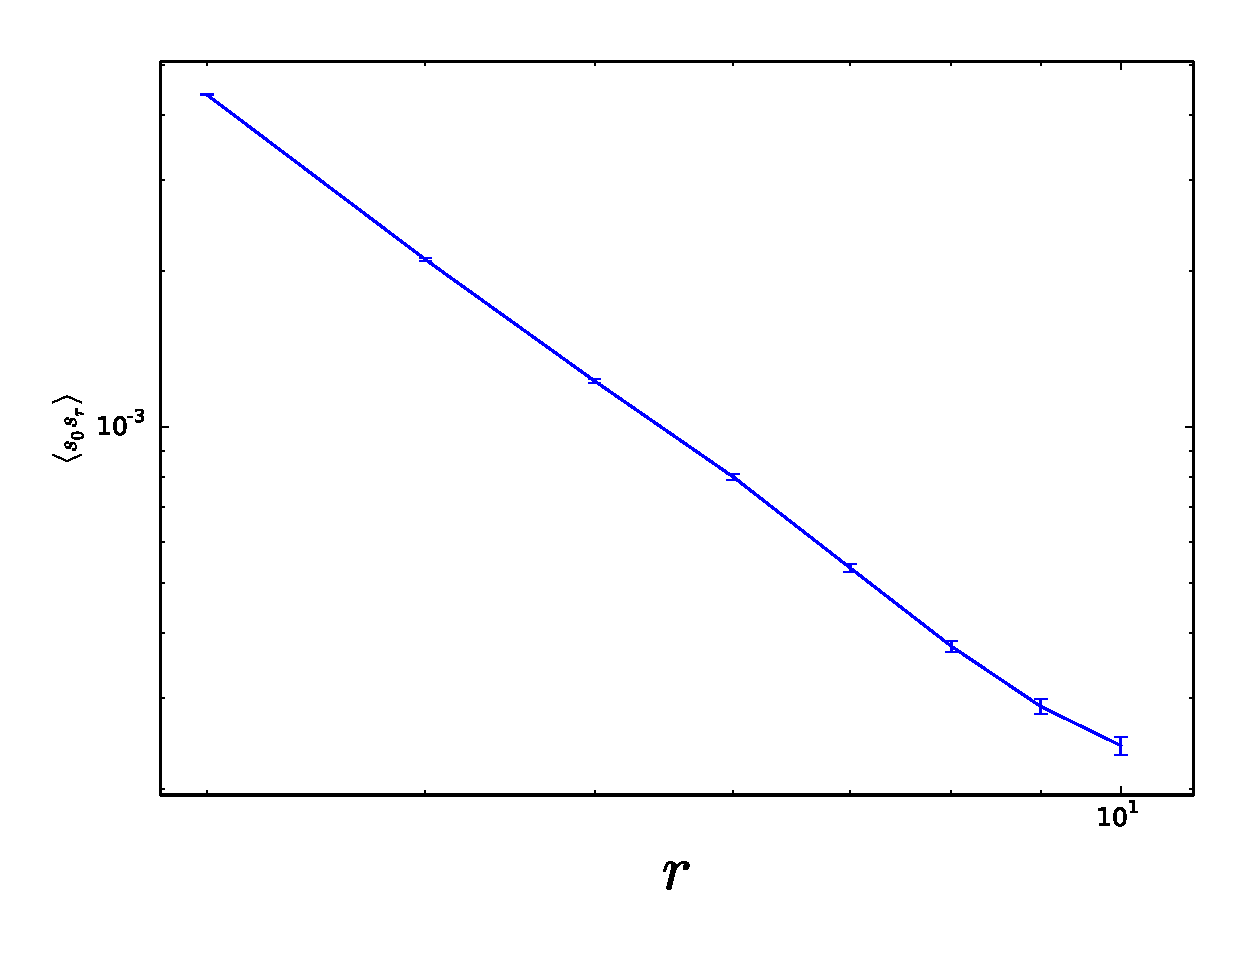
\includegraphics[width=8.5 cm]{fit_dm_dm_horz_ln_pnts_64x64}
    \caption{The points chosen from fig \ref{fig:dimer_dimer_cor_log} that are used to calculate the
    slope.\label{fig:fit_dm_dm_64x64}}
\end{figure}

\begin{figure}[h]
    \centering
    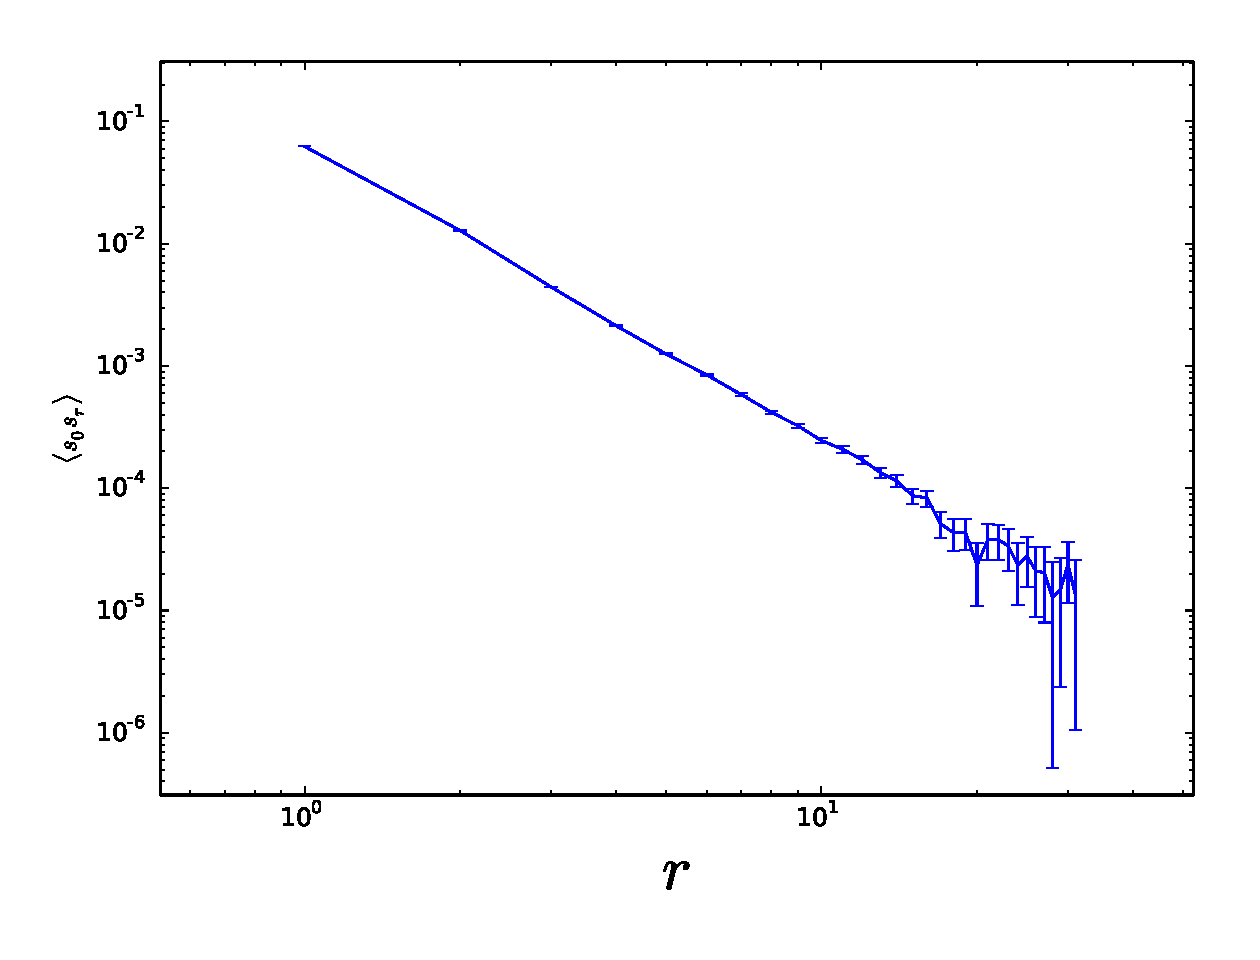
\includegraphics[width=8.5 cm]{dimer_dimer_cor_log_128x128}
    \caption{The log log plot of the points used to calculate the sope of the dimer dimer
        correlation function on a $128\times 128$ lattice. Number of bins: 9,000. Each bin is
    averaged over 500,000 measurments\label{fig:dimer_dimer_cor_log_128x128}}
\end{figure}

\begin{figure}[h]
    \centering
    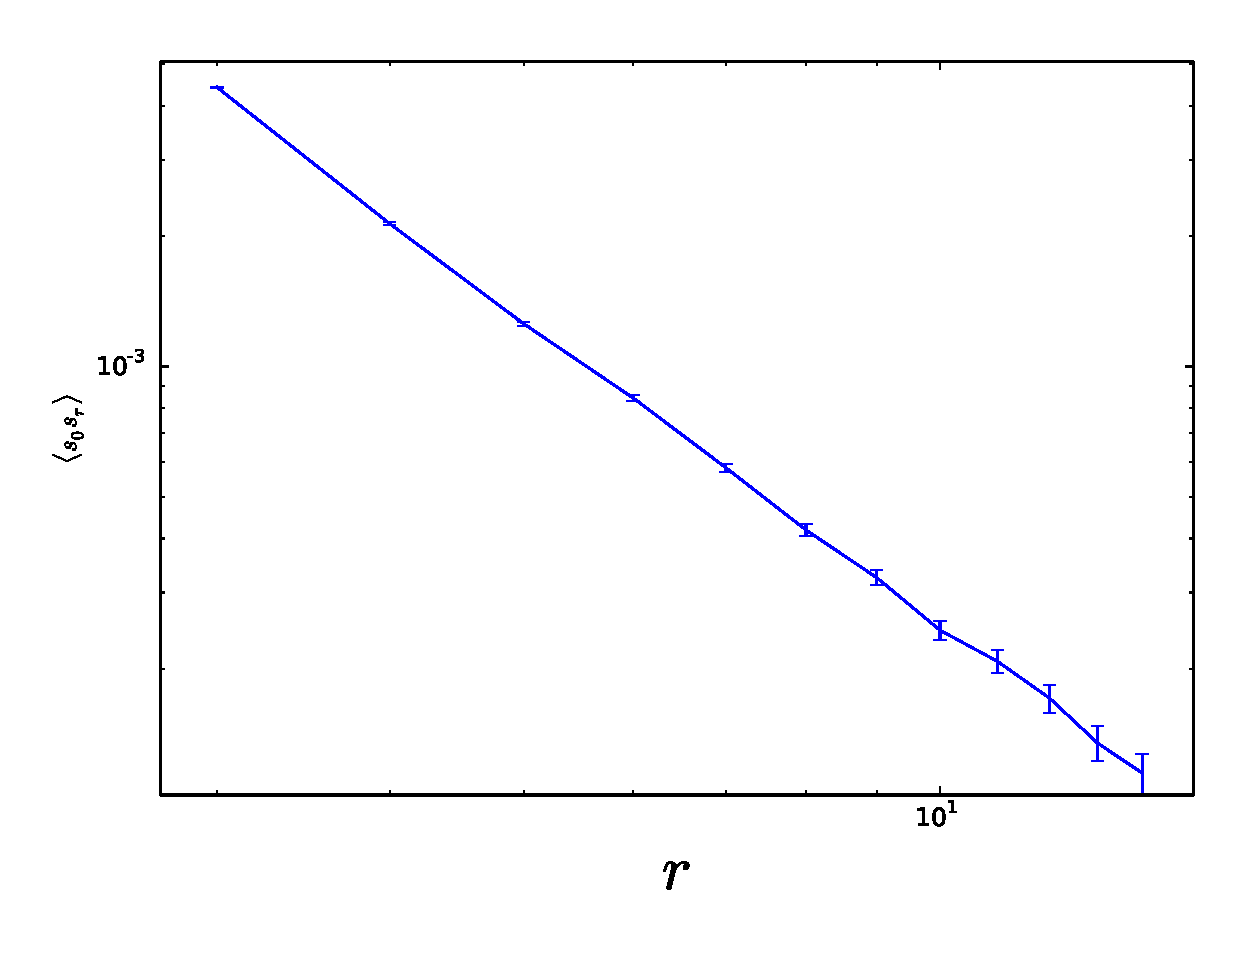
\includegraphics[width=8.5 cm]{fit_dm_dm_horz_ln_pnts_128x128}
    \caption{The points used in the fit for the $128\times128$ lattice.\label{fig:fit_dm_dm_128x128}}
\end{figure}

\begin{figure}[h]
    \centering
    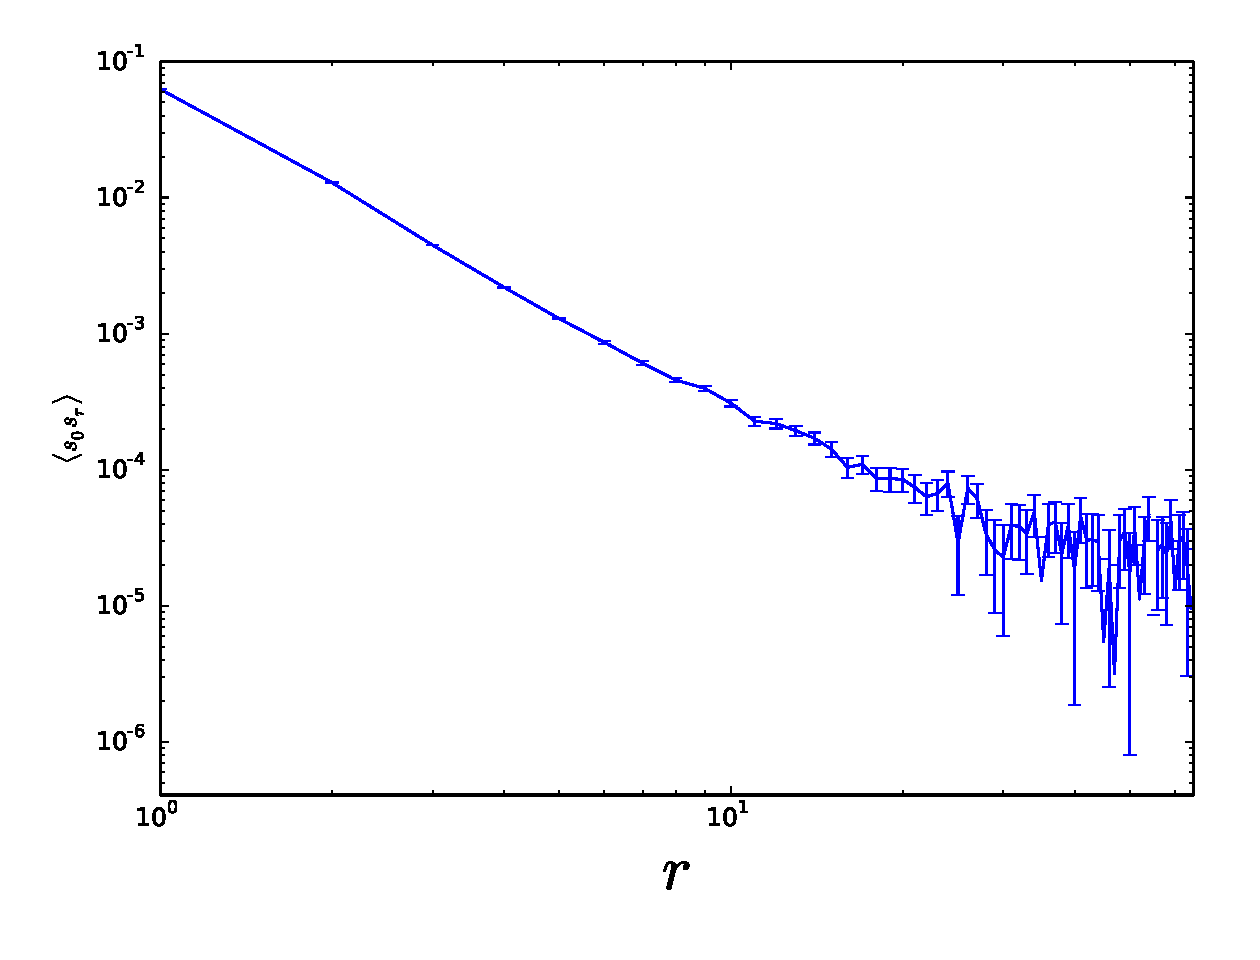
\includegraphics[width=8.5 cm]{dimer_dimer_cor_log_256x256}
    \caption{The log log plot of the points used to calculate the sope of the dimer dimer
        correlation function on a $256\times 256$ lattice. Number of bins: 9,000. Each bin is
    averaged over 500,000 measurments\label{dimer_dimer_cor_log_256x256}}
\end{figure}

\begin{figure}[h]
    \centering
    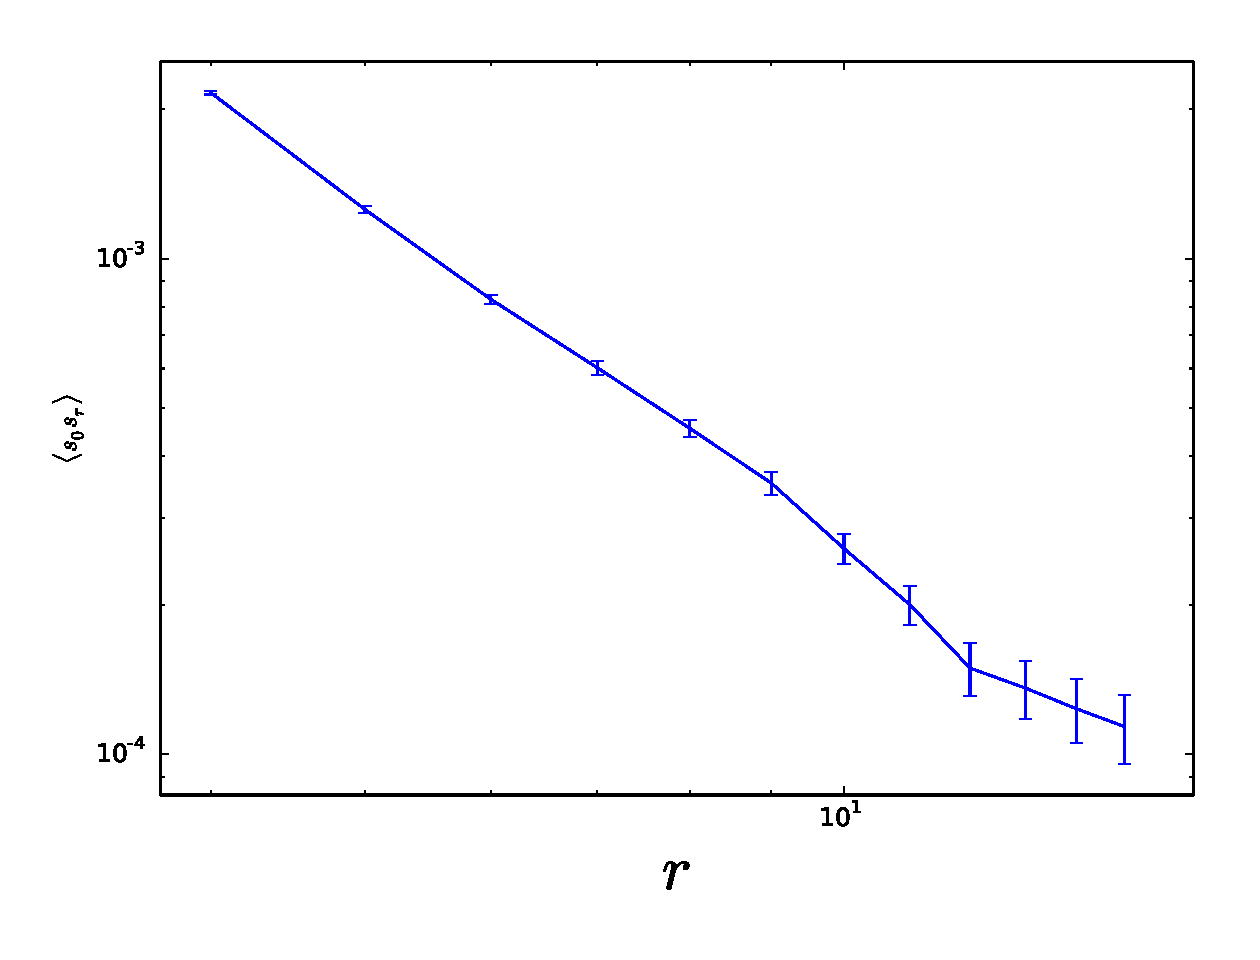
\includegraphics[width=8.5 cm]{fit_dm_dm_horz_ln_pnts_256x256}
    \caption{The points used in the fit for the $256\times256$ lattice.\label{fig:fit_dm_dm_256x256}}
\end{figure}

\clearpage
%%%%%%%%%%%%%%%%%%%%%%%%%%%%%%%%%%%%%%%%%%%%%%%%%%%%%%%%%%%%%%%%%%%%%%%%%%%%%%%%%%%%%%%%%%%%%%%%%%%%%%%%%%%%%%%%%%%%%%%%%%
%%%%%%%%%%%%%%%%%%%%%%%%%%%%%%%%%%%%%%%%%%%%%%%%%%%%%%%%%%%%%%%%%%%%%%%%%%%%%%%%%%%%%%%%%%%%%%%%%%%%%%%%%%%%%%%%%%%%%%%%%%
%%%%%%%%%%%%%%%%%%%%%%%%%%%%%%%%%%%%%%%%%%%%%%%%%%%%%%%%%%%%%%%%%%%%%%%%%%%%%%%%%%%%%%%%%%%%%%%%%%%%%%%%%%%%%%%%%%%%%%%%%%
%%%%%%%%%%%%%%%%%%%%%%%%%%%%%%%%%%%%%%%%%%%%%%%%%%%%%%%%%%%%%%%%%%%%%%%%%%%%%%%%%%%%%%%%%%%%%%%%%%%%%%%%%%%%%%%%%%%%%%%%%%

\section{Star Dimer}

Very preliminary results of the star star correlation function are shown in fig.
\ref{fig:star_star_cor}. 

\begin{equation}
    \label{}
    C_{star}(0,r) =  \langle star_0 star_r \rangle -\langle star_0 \rangle \langle star_r \rangle
\end{equation}

\noindent
The disconnected piece has been numerically measured for a couple of different lattice sizes shown
in table \ref{table:counts}.

\begin{figure}[h]
    \centering
    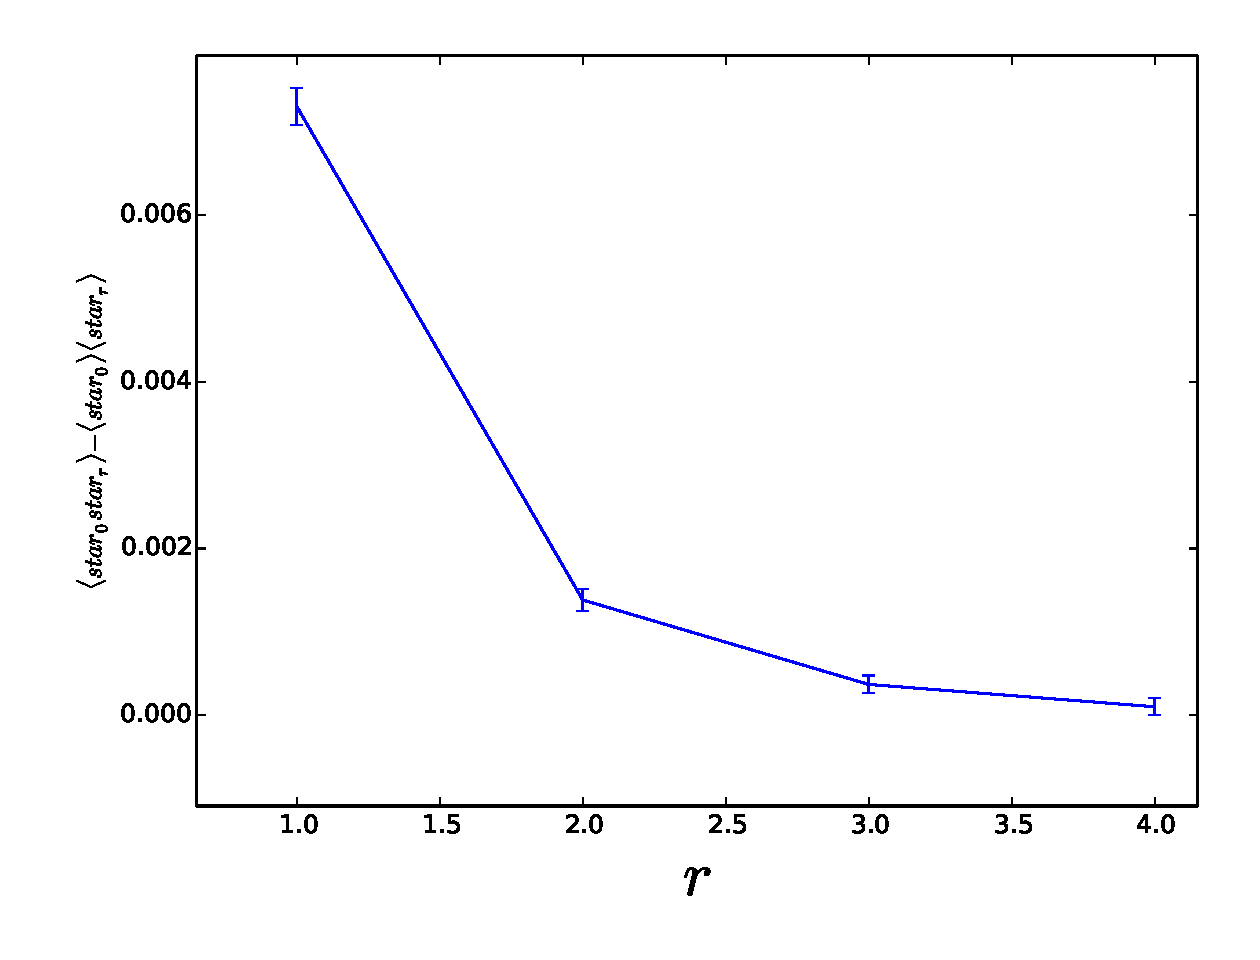
\includegraphics[width=8.5 cm]{star_star_cor}
    \caption{Star star correlation function (just along y direction) \label{fig:star_star_cor}}
\end{figure}

\begin{figure}[h]
    \centering
    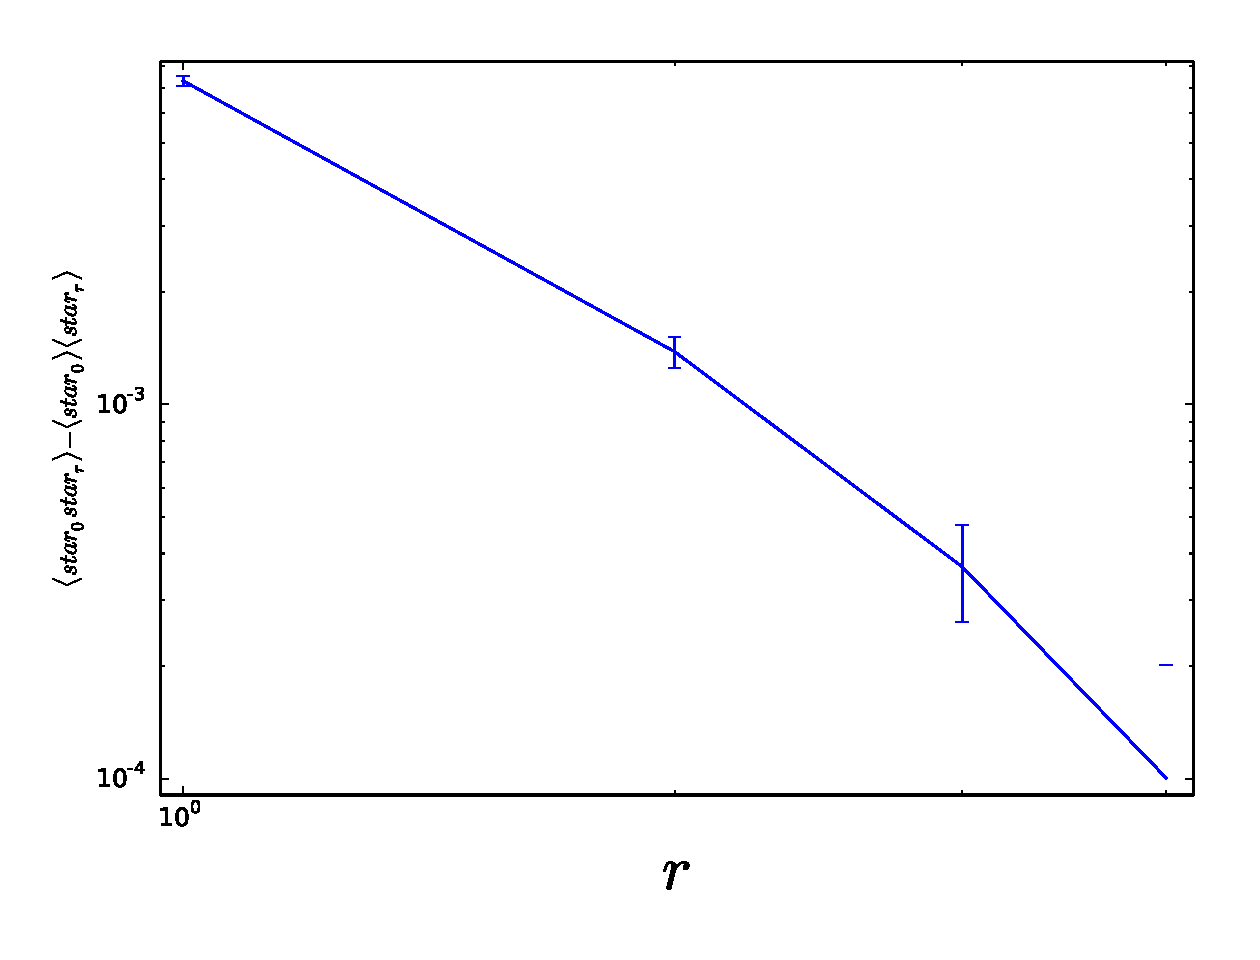
\includegraphics[width=8.5 cm]{star_star_cor_log}
    \caption{Star star correlation function (just along y direction) log log plot.\label{fig:star_star_cor_log}}
\end{figure}

\begin{figure}[h]
    \centering
    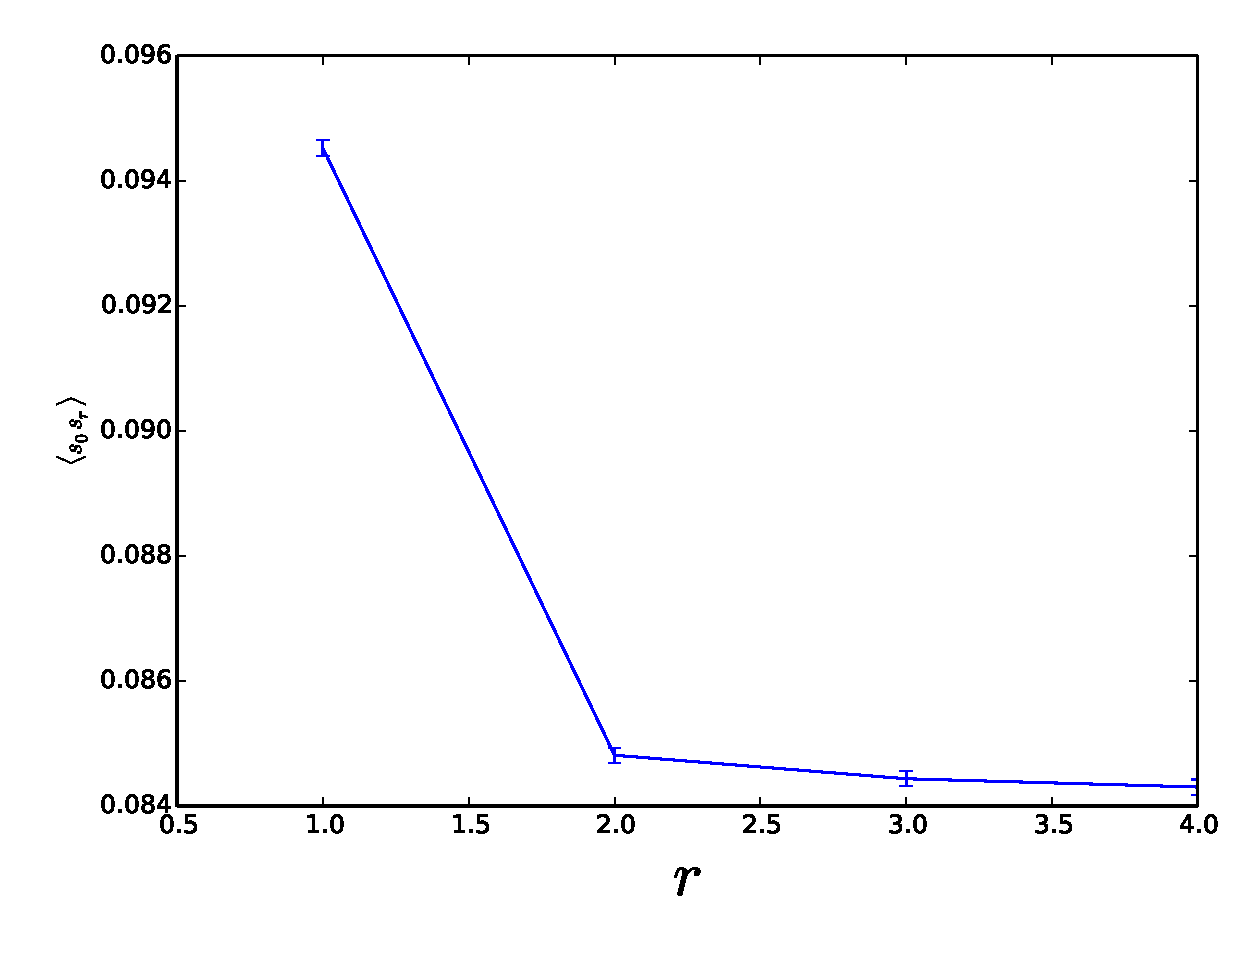
\includegraphics[width=8.5 cm]{s_dimer_dimer_cor}
    \caption{Dimer dimer correlation function in the star dimer model \label{fig:s_dimer_dimer}}
\end{figure}

\clearpage
%%%%%%%%%%%%%%%%%%%%%%%%%%%%%%%%%%%%%%%%%%%%%%%%%%%%%%%%%%%%%%%%%%%%%%%%%%%%%%%%%%%%%%%%%%%%%%%%%%%%%%%%%%%%%%%%%%%%%%%%%%
%%%%%%%%%%%%%%%%%%%%%%%%%%%%%%%%%%%%%%%%%%%%%%%%%%%%%%%%%%%%%%%%%%%%%%%%%%%%%%%%%%%%%%%%%%%%%%%%%%%%%%%%%%%%%%%%%%%%%%%%%%
\subsection{Star Pair Creation and Annihilation}

Creation and annihilation of a horizontal pair of stars is shown in fig.
\ref{fig:create_annihilate_pair}. Creation and annihilation of a vertical pair of stars can be
is simply what is shown in fig. \ref{fig:create_annihilate_pair} rotated by $\pi/2$.

\begin{figure}[h]
    \centering
    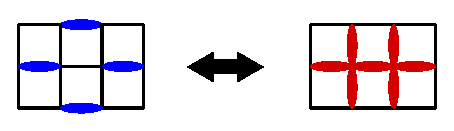
\includegraphics[width=8.5 cm]{create_annihilate_pair}
    \caption{The creation and annihilation of a pair of stars.
\label{fig:create_annihilate_pair}}
\end{figure}

\subsection{Star Horizontal/Vertical Translation}
Horizontal translations of a star is shown in fig. \ref{fig:move_right_left}. The vertical
translations can be obtained by rotating fig. \ref{fig:move_right_left} by $\pi/2$. Horizontal
translations must be preformed such that the star remains on its original sub-lattice, thus the
minimal translation is by two vertices.

\begin{figure}[h]
    \centering
    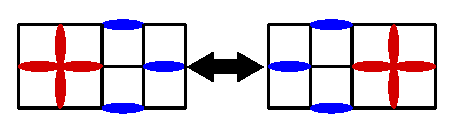
\includegraphics[width=8.5 cm]{move_right_left}
    \caption{Horizontal translation of a star.
\label{fig:move_right_left}}
\end{figure}


\subsection{Star Diagonal Translation}
A star can remain on its original sub-lattice through a diagonal translation as well. We show a star moving
to the lower right diagonal in fig. \ref{fig:diag}. 
\begin{figure}[h]
    \centering
    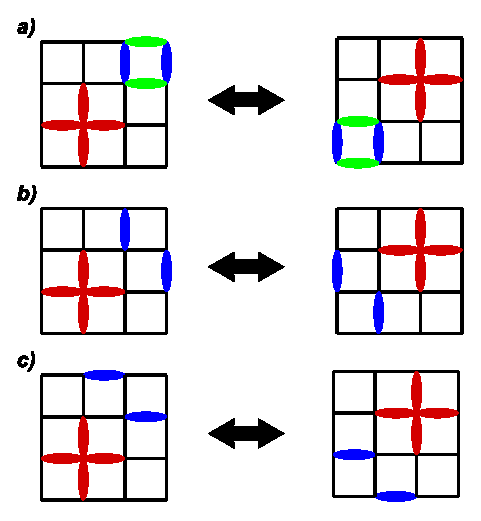
\includegraphics[width=8.5 cm]{diag}
    \caption{Diagonal translation to the lower right diagonal.
\label{fig:diag}}
\end{figure}

\clearpage
%%%%%%%%%%%%%%%%%%%%%%%%%%%%%%%%%%%%%%%%%%%%%%%%%%%%%%%%%%%%%%%%%%%%%%%%%%%%%%%%%%%%%%%%%%%%%%%%%%%%%%%%%%%%%%%%%%%%%%%%%%
%%%%%%%%%%%%%%%%%%%%%%%%%%%%%%%%%%%%%%%%%%%%%%%%%%%%%%%%%%%%%%%%%%%%%%%%%%%%%%%%%%%%%%%%%%%%%%%%%%%%%%%%%%%%%%%%%%%%%%%%%%
\subsection{Autocorrelation Time}

\begin{figure}[h]
    \centering
    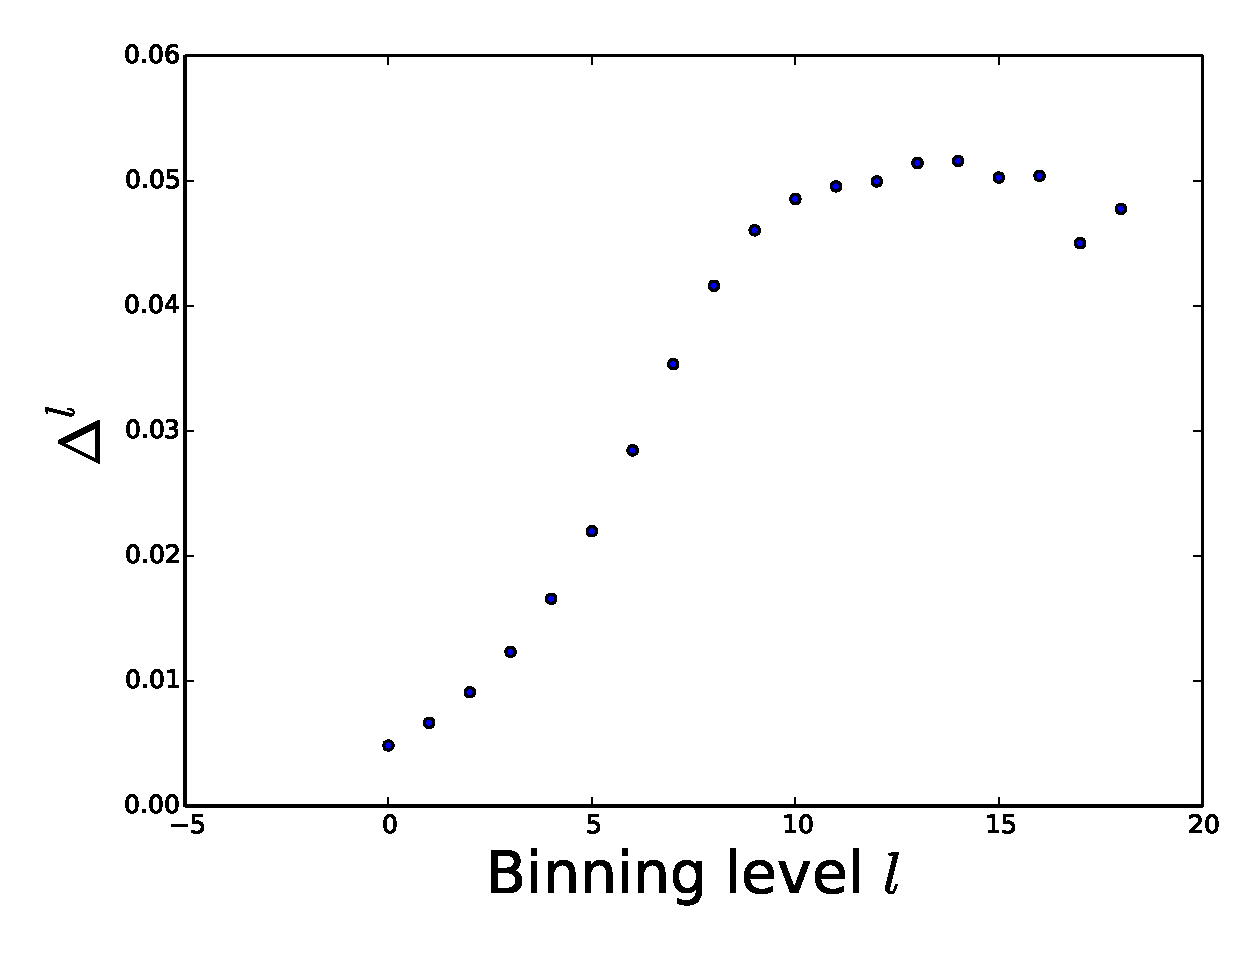
\includegraphics[width=8.5 cm]{auto_cor_num_stars}
    \caption{Autocorrelation time for the number of stars on a $32\times 32$ lattice. Binning was preformed on $4\times 10^6$
    measurements each spaced $t_{mc}$. \label{fig:auto_cor_num_stars}}
\end{figure}

\begin{figure}[h]
    \centering
    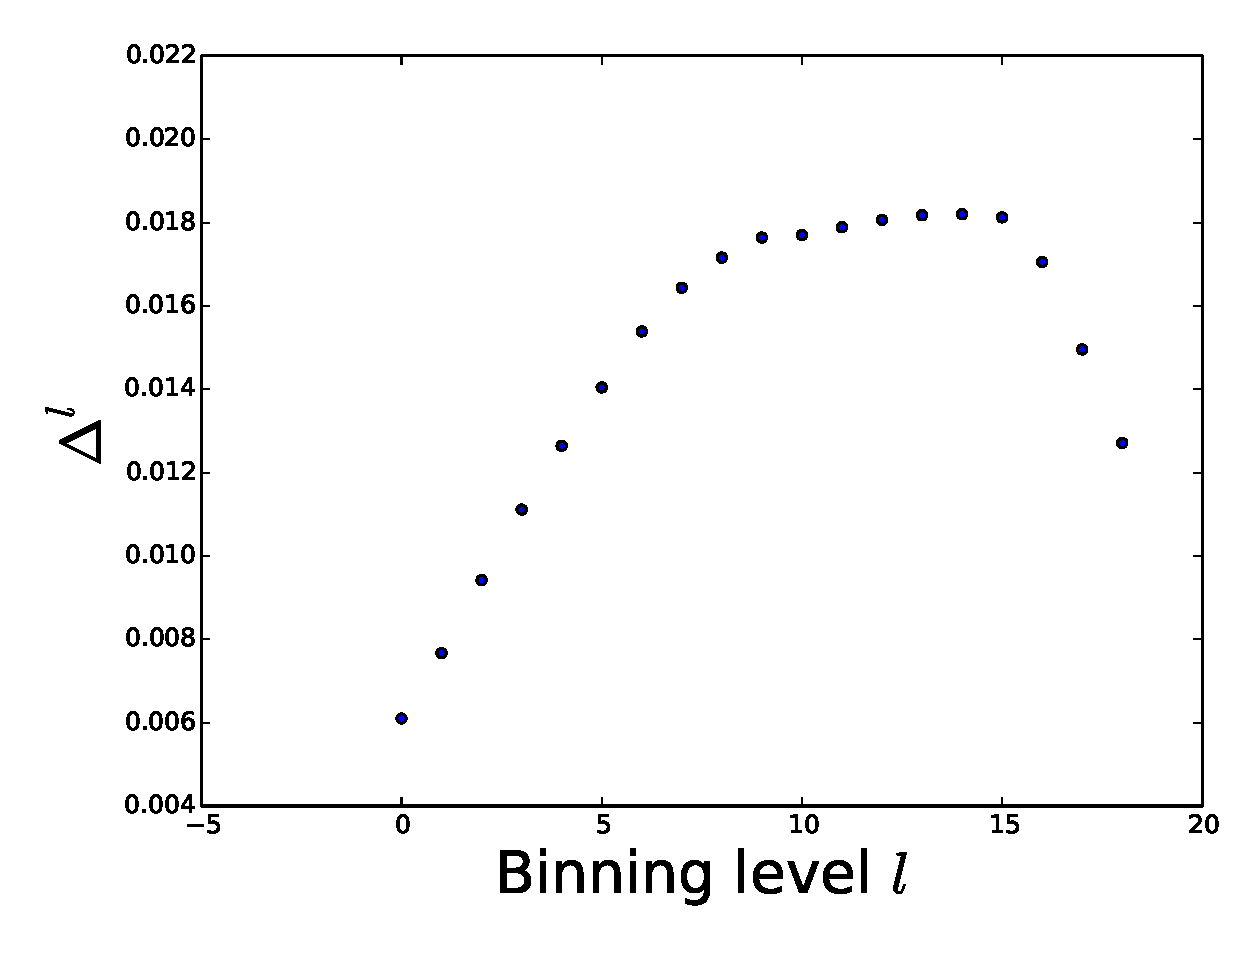
\includegraphics[width=8.5 cm]{auto_cor_num_horz}
    \caption{Autocorrelation time for the number of horizontal dimers on a $32\times 32$ lattice. Binning was preformed on $4\times 10^6$
    measurements each spaced $t_{mc}$. \label{fig:auto_cor_num_stars}}
\end{figure}

\begin{figure}[h]
    \centering
    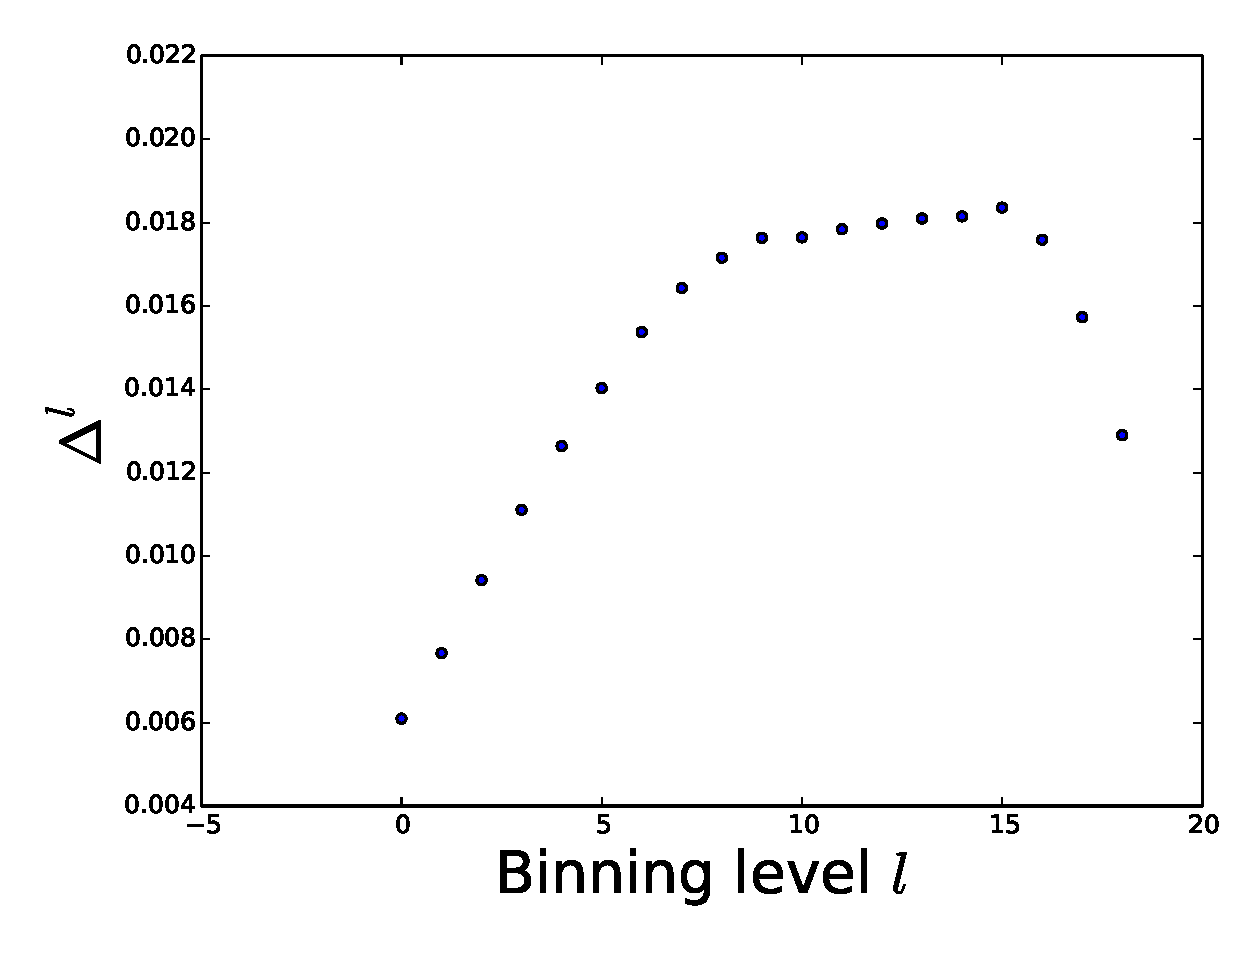
\includegraphics[width=8.5 cm]{auto_cor_num_vert}
    \caption{Autocorrelation time for the number of vertical dimers on a $32\times 32$ lattice. Binning was preformed on $4\times 10^6$
    measurements each spaced $t_{mc}$. \label{fig:auto_cor_num_stars}}
\end{figure}

\clearpage
\subsection{Equilibration Time}

We show three order parameters as a function of Monte Carlo time, $t_{mc}$: 

\begin{itemize}
    \item The number of stars.
    \item The difference between the number of vertical dimers and horizontal dimers.
    \item The number of flippable plaquetts.
\end{itemize}

\noindent
in fig. \ref{fig:nums_of_things}. We define $t_{mc}$ to be $2lh$ local updates, where $l$ is the length of the system and $h$ is the
height of the system in number of vertices. This lattice size used was $64\times 64$. Each data
point shown is the average over 100 different simulations. The error bars are the standard deviations of
the counts used in taking the mean. It appears as if the equilibration time is around $400t_{mc}$. 

\begin{figure}[h]
    \centering
    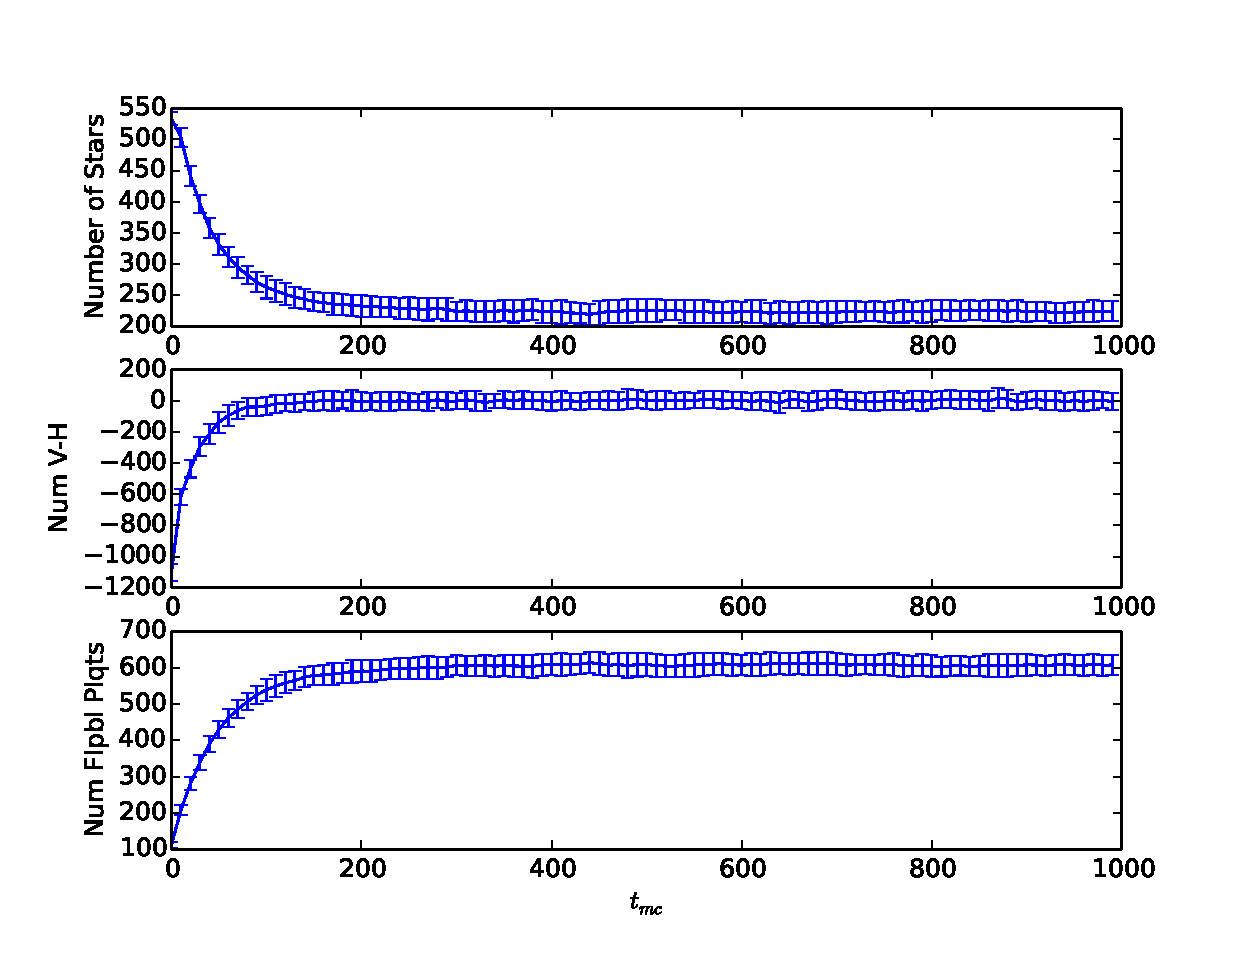
\includegraphics[width=8.5 cm]{num_order_params}
    \caption{From the top down: The number of stars on the lattice, the difference between the
    number of vertical dimers and horizontal dimers, and the number of flippable plaquetts as a
    function of Monte Carlo time $t_{mc}$. \label{fig:nums_of_things}}
\end{figure}

%\subsection{Autocorrelation time}
%
%\begin{figure}[h]
%    \centering
%    \includegraphics[width=8.5 cm]{}
%    \caption{A binning analysis preformed on ###### bins, where each bin is an average over 100
%    measurements and each measurement was taken after one $t_{mc} \label{fig:}}
%\end{figure}

\subsection{Star Concentrations}

The following statistics are given for different lattice sizes but each set of data is found using
100,000 bins, each an average over 10 measurements, each measurement taken after $1\times t_{mc}$.
We have not included the first 400 $t_{mc}$ so that the averages are found in an equilibrated
system.

\begin{table}[htp]
    \caption{Some Counting}
    \centering
    \begin{tabular}{l | l | l | l}
    \hline\hline
    lattice size                                            & $16\times 16$ & $32\times 32$   & $64\times 64$ \\ \hline
    $\langle \# stars \rangle$                              &               &  $55.66655$     & $ 222.51807 $\\ \hline
    $\sigma_{\# stars}$                                     &               &  $9.67847$      & $ 17.23504  $\\ \hline
    $\langle star_{i,j} \rangle$                            &               &  $0.05436$      & $ 0.05432   $\\ \hline
    $\langle star_{i,j} \rangle \langle star_{i,j} \rangle$ &               &  $0.00296$      & $ 0.00295   $\\ \hline 
    \hline
    $\langle \# - \rangle$                                  &               &$256.02732$      & \\ \hline
    $\sigma_{\# -}$                                         &               & $12.20027$      & \\ \hline
    $\langle -_{i,j} \rangle$                               &               &  $0.25003$      & \\ \hline
    $\langle star_{i,j} \rangle \langle star_{i,j} \rangle$ &               &  $0.06251$      & \\ \hline
    \hline
    $\langle \# \| \rangle$                                 &               &$255.97332$      & \\ \hline
    $\sigma_{\# \|}$                                        &               & $12.19720$      & \\ \hline
    $\langle \|_{i,j} \rangle$                              &               &  $0.24997$      & \\ \hline
    $\langle \|_{i,j} \rangle \langle \|_{i,j} \rangle$     &               &  $0.06249$      & \\ \hline \\ [1ex]
    \end{tabular}
    \label{table:counts}
\end{table}


\clearpage
\subsection{Translational Symmetry Breaking}

On an $8\times 8$ lattice we find that there is always some residual asymmetry in the horizontal
dimers (speculation:) due to the initial configuration of dimers. This appears to be an effect of
small system size as the $16\times 16$ lattice looks to be transnationally invariant.

\begin{figure}[h]
    \centering
    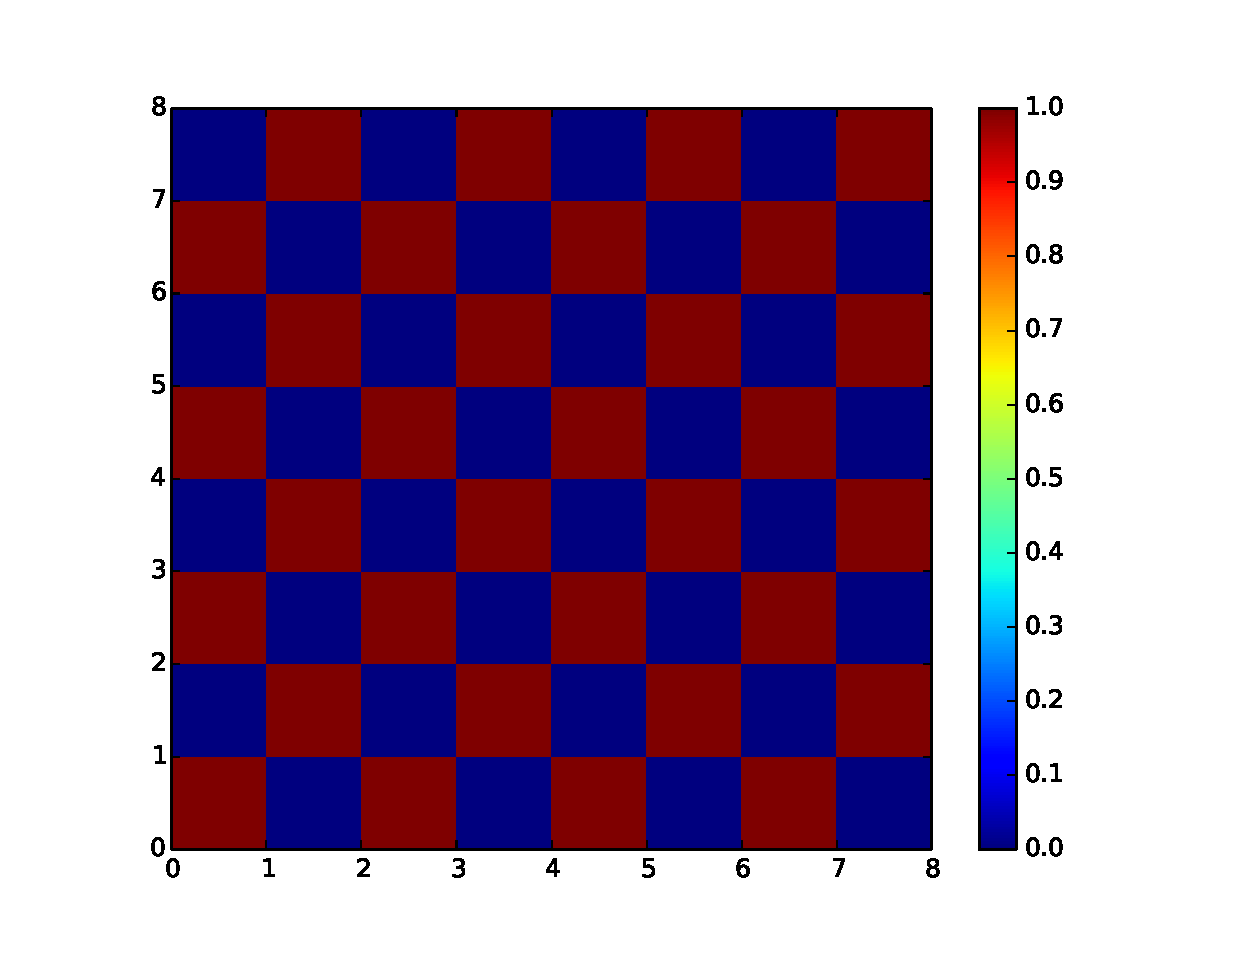
\includegraphics[width=8.5 cm]{grey_scale_init_config_horz}
    \caption{Heat map of horizontal dimer placement in the initial staggered configuration of the
    lattice. Lattice size: $8\times 8$ \label{fig:horz_init_heat}}
\end{figure}


\begin{figure}[h]
    \centering
    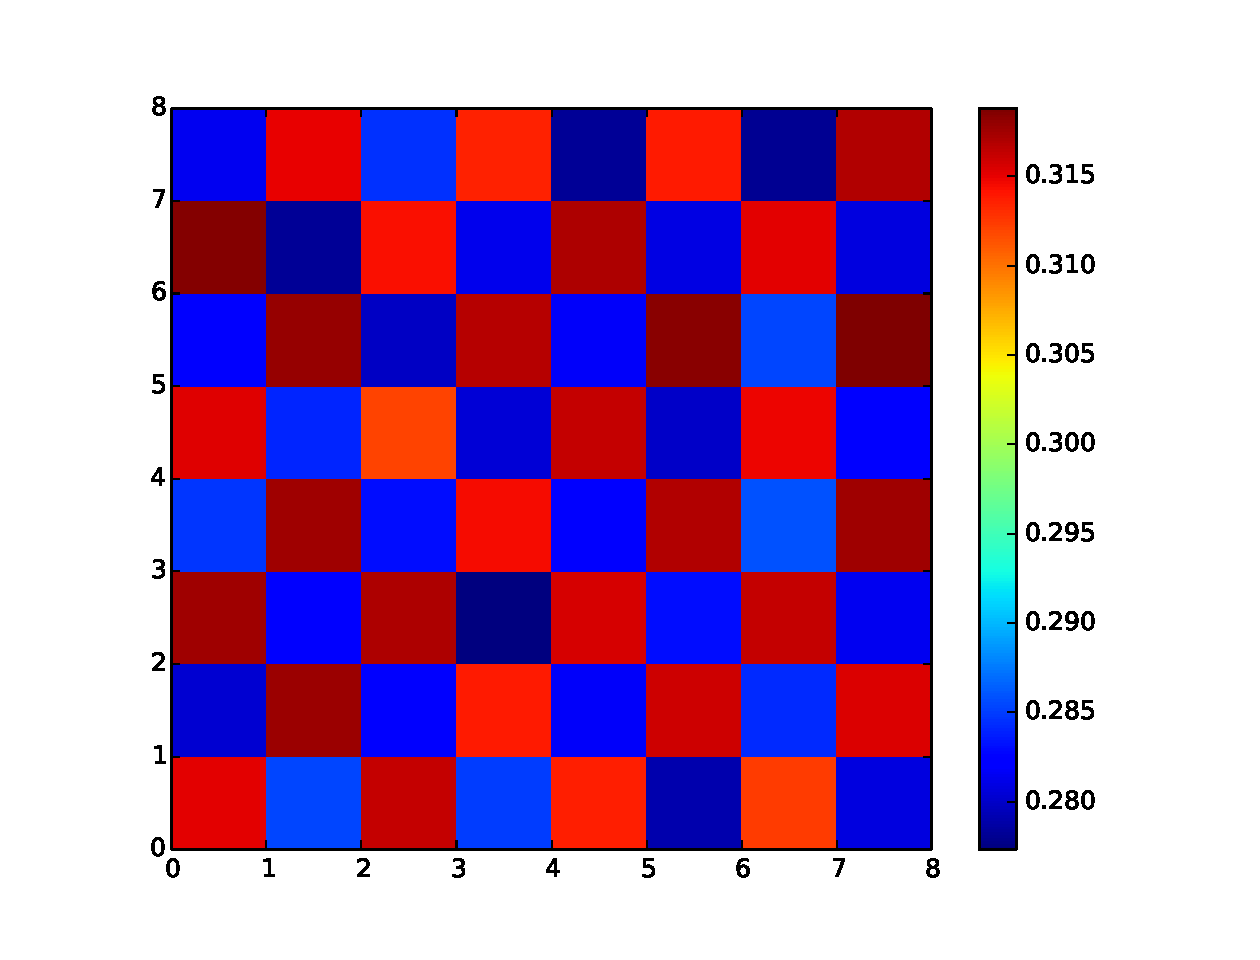
\includegraphics[width=8.5 cm]{grey_scale_avg_horz}
    \caption{Heat map of horizontal dimer placement on an $8\times 8$ lattice. Each representing the
        occupation (red) and absence (blue) of a horizontal dimer is averaged over 50,000 configurations. Each
        configuration included in the average is separated by $100t_{mc}$. Time passed before
        collecting data was $5\times 10^6 t_{mc}$.  \label{fig:horz_avg_heat}}
\end{figure}

\begin{figure}[h]
    \centering
    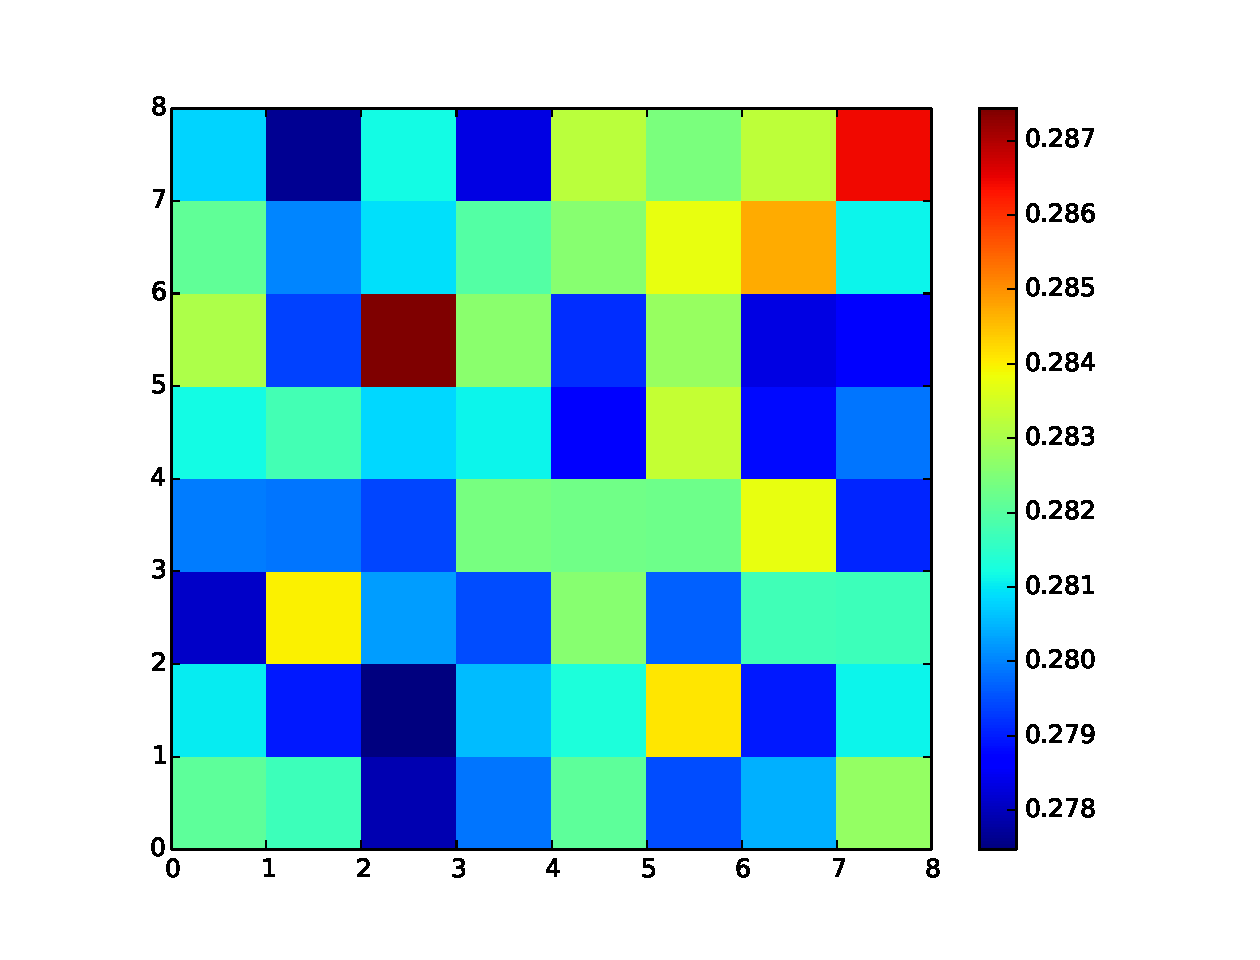
\includegraphics[width=8.5 cm]{grey_scale_avg_vert}
    \caption{Heat map of horizontal dimer placement on an $8\times 8$ lattice. Each representing the
        occupation (red) and absence (blue) of a horizontal dimer is averaged over 50,000 configurations. Each
        configuration included in the average is separated by $100t_{mc}$. Time passed before
        collecting data was $5\times 10^6 t_{mc}$. \label{fig:vert_avg_heat}}
\end{figure}


\begin{figure}[h]
    \centering
    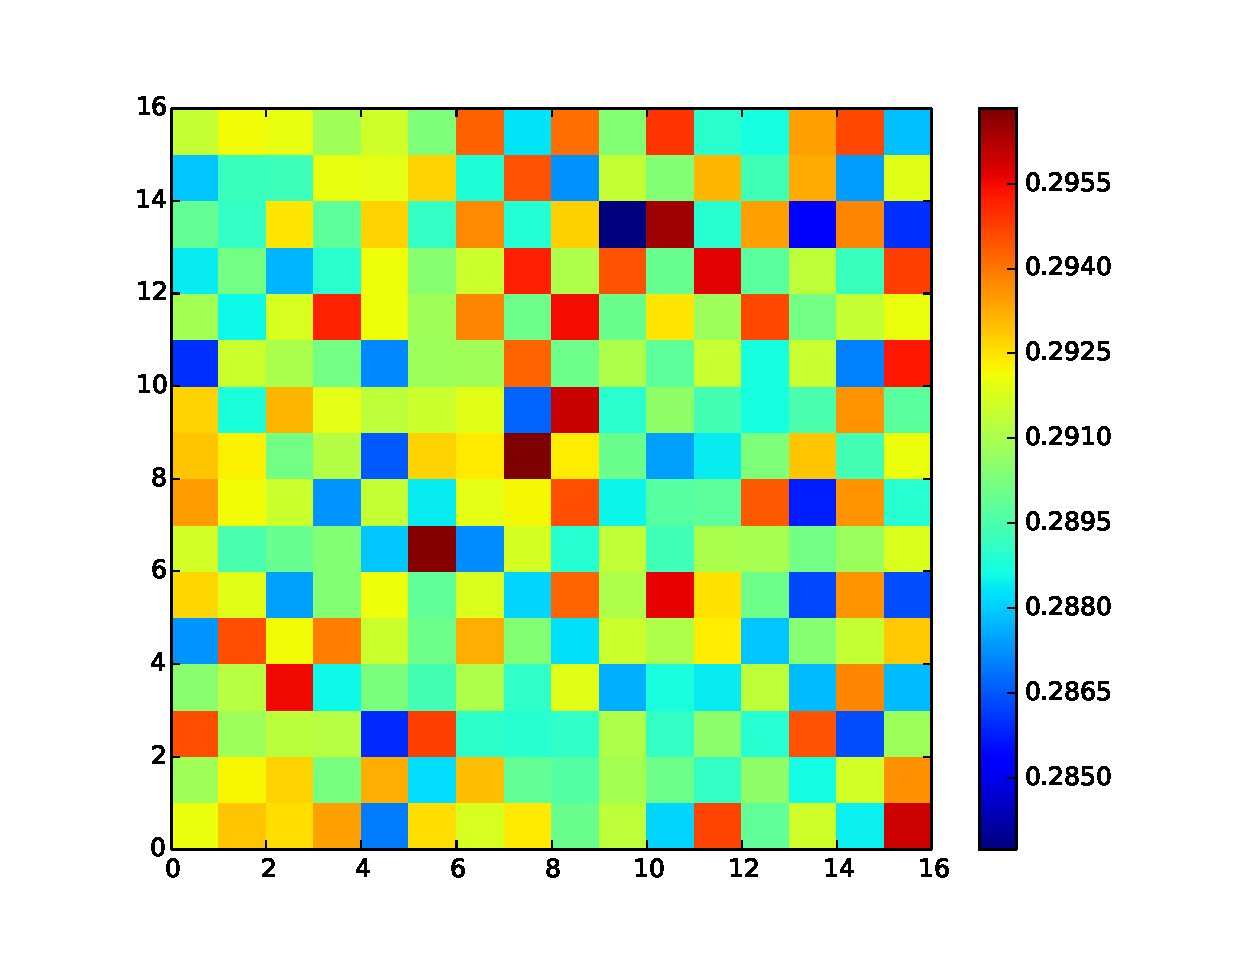
\includegraphics[width=8.5 cm]{grey_scale_avg_horz_16x16}
    \caption{Heat map of horizontal dimer placement on an $16\times 16$ lattice. Each representing the
        occupation (red) and absence (blue) of a horizontal dimer is averaged over 50,000 configurations. Each
        configuration included in the average is separated by $100t_{mc}$. Time passed before
        collecting data was $5\times 10^6 t_{mc}$. \label{fig:horz_avg_heat_16x16}}
\end{figure}

\begin{figure}[h]
    \centering
    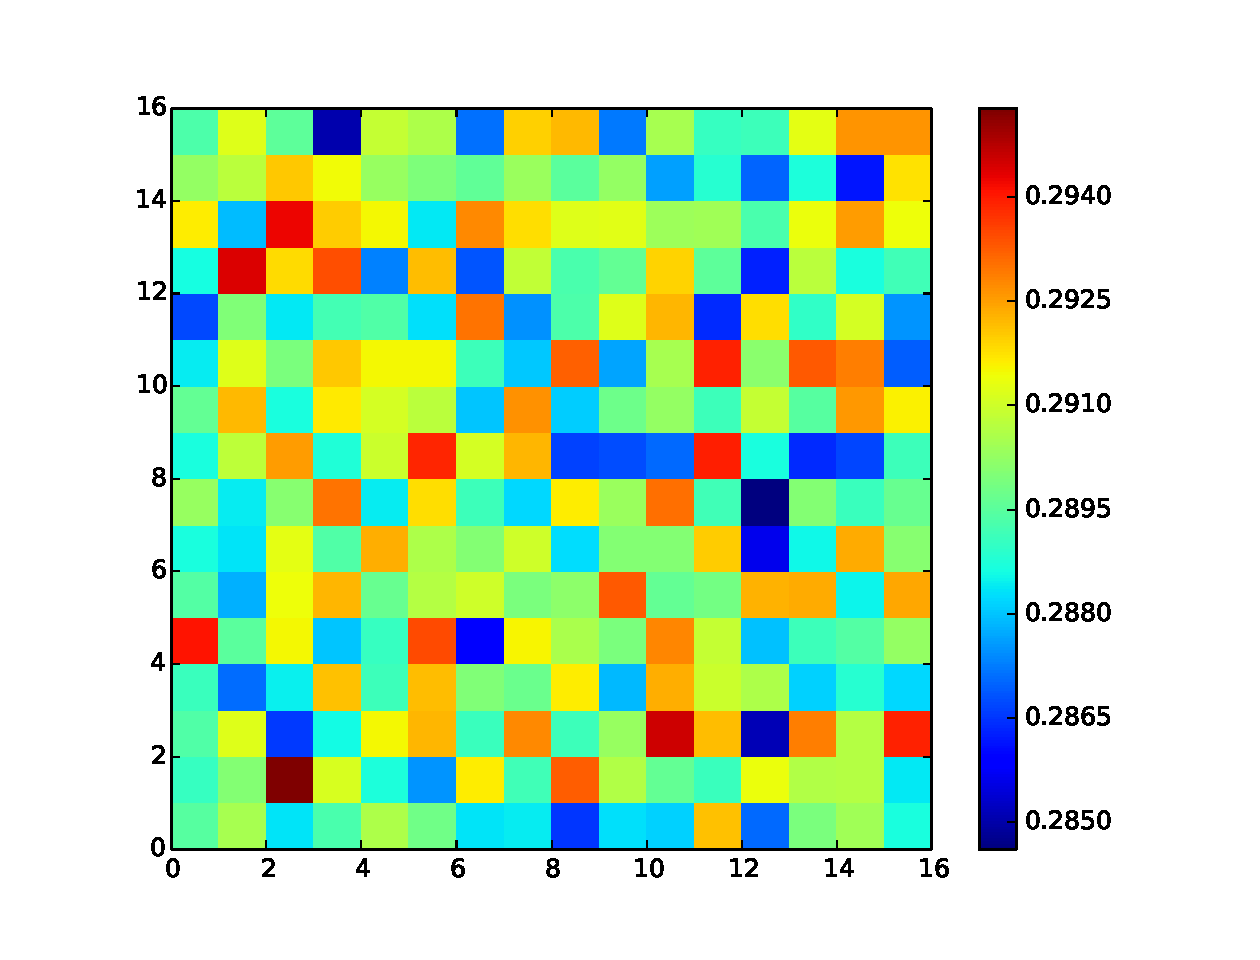
\includegraphics[width=8.5 cm]{grey_scale_avg_vert_16x16}
    \caption{Heat map of vertical dimer placement on an $16\times 16$ lattice. Each representing the
        occupation (red) and absence (blue) of a vertical dimer is averaged over 50,000 configurations. Each
        configuration included in the average is separated by $100t_{mc}$. $5\times 10^6 t_{mc}$ passed
        before collecting data. \label{fig:vert_avg_heat_16x16}}
\end{figure}


\clearpage
%%%%%%%%%%%%%%%%%%%%%%%%%%%%%%%%%%%%%%%%%%%%%%%%%%%%%%%%%%%%%%%%%%%%%%%%%%%%%%%%%%%%%%%%%%%%%%%%%%%%%%%%%%%%%%%%%%%%%%%%%%
%%%%%%%%%%%%%%%%%%%%%%%%%%%%%%%%%%%%%%%%%%%%%%%%%%%%%%%%%%%%%%%%%%%%%%%%%%%%%%%%%%%%%%%%%%%%%%%%%%%%%%%%%%%%%%%%%%%%%%%%%%
\subsection{Old Moves and Rules}

Creating a pair of stars in the staggered state is shown in fig. \ref{fig:old_create_pair}. We notice
the creation of a star produces two flippable plaquettes between the two stars.

\begin{figure}[h]
    \centering
    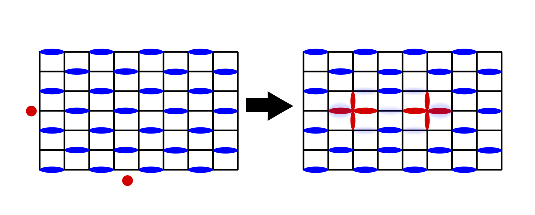
\includegraphics[width=8.5 cm]{old_create_pair}
    \caption{The creation of a pair of stars in the fully packed staggered configuration. The red
    dots on the $x$ and $y$ axes show the dimer about which the stars are created.
\label{fig:old_create_pair}}
\end{figure}

\noindent In fig. \ref{fig:old_move_right} we show the rightmost star move right in the same
configuration. In any single star must remain on the sublattice it was created on, so the center of
the star moves by two vertices. We notice that the horizontal propagation of a star creates two boundaries of
flippable plaquettes across the top and bottom of the star pair. 

\begin{figure}[h]
    \centering
    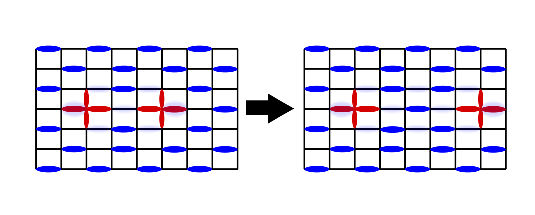
\includegraphics[width=8.5 cm]{old_move_right}
    \caption{The move of the rightmost star in fig. \ref{fig:old_create_pair} \label{fig:old_move_right}}
\end{figure}

Still figuring out the possible ways to move stars vertically. In six steps we show it is possible
to implement a specific type of local vertical move. 
\\

\begin{itemize}
    \item 
    Step 1 (fig. \ref{fig:ex_vert_mv_1}): create a pair of stars.
    
    \item 
    Step 2 (fig. \ref{fig:ex_vert_mv_2}): Move rightmost star right four times creating a horizontal set of
    flippable plaquettes.
    
    \item
    Step 3 (fig. \ref{fig:ex_vert_mv_3}): Flip some of the plaquettes. 
    
    \item
    Step 4 (fig. \ref{fig:ex_vert_mv_4}): With several vertical pairs of dimers we can flip on plaquette to make a
    horizontal pair that was not part of the original set of horizontal dimers after the star move. The
    $x$ and $y$ positions of this plaquette are marked in fig. \ref{fig:ex_vert_mv_4} by red dots along the $x$ and $y$
    axes. If all of the dimers were left as vertical or horizontal the move would not be possible.
    
    \item
    Step 5 (fig. \ref{fig:ex_vert_mv_5}): Create another pair of stars.
    
    \item
    Step 6 (fig. \ref{fig:ex_vert_mv_6}): Move the rightmost star of the new pair up. When this is done
    the dimers must be rearranged to satisfy the packing conditions and conserve the number of dimers.
    Right now this is the only configuration I see for this move that can satisfy these conditions.
\end{itemize}


\begin{figure}[h]
    \centering
    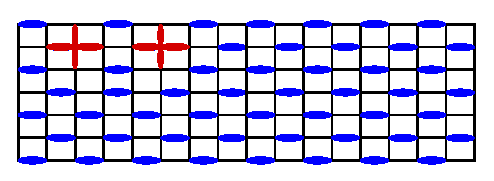
\includegraphics[width=8.5 cm]{ex_vert_mv_1}
    \caption{Step 1 in the vertical move example. Create a pair of stars.\label{fig:ex_vert_mv_1}}
\end{figure}

\begin{figure}[h]
    \centering
    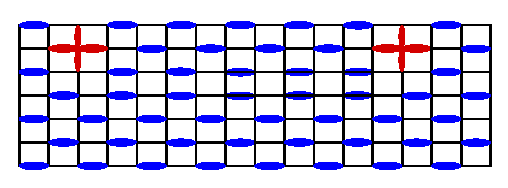
\includegraphics[width=8.5 cm]{ex_vert_mv_2}
    \caption{Step 2 in the vertical move example. Move the rightmost star right four times creating
    a horizontal set of flippable plaquettes.\label{fig:ex_vert_mv_2}}
\end{figure}

\begin{figure}[h]
    \centering
    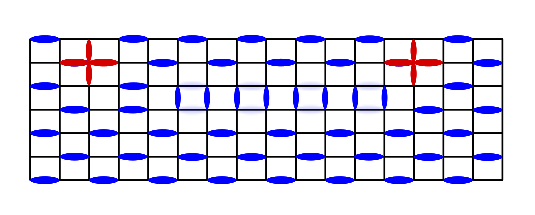
\includegraphics[width=8.5 cm]{ex_vert_mv_3}
    \caption{Step 3 in the vertical move example. Flip some of the plaquettes.\label{fig:ex_vert_mv_3}}
\end{figure}


\begin{figure}[h]
    \centering
    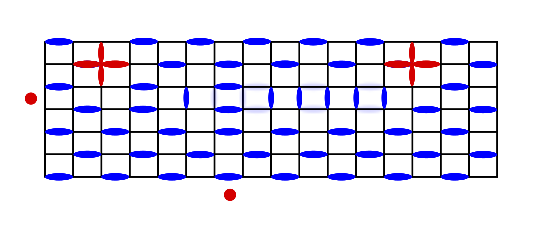
\includegraphics[width=8.5 cm]{ex_vert_mv_4}
    \caption{Step 4 in the vertical move example. Flip the plaquette at the $x$ and $y$ coordinates
    marked by the red dots.\label{fig:ex_vert_mv_4}}
\end{figure}


\begin{figure}[h]
    \centering
    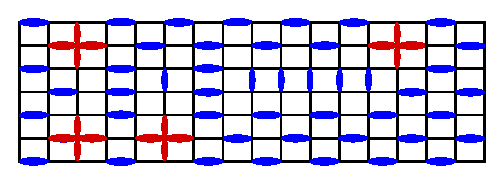
\includegraphics[width=8.5 cm]{ex_vert_mv_5}
    \caption{Step 5 in the vertical move example. Create another pair of stars.\label{fig:ex_vert_mv_5}}
\end{figure}

\begin{figure}[h]
    \centering
    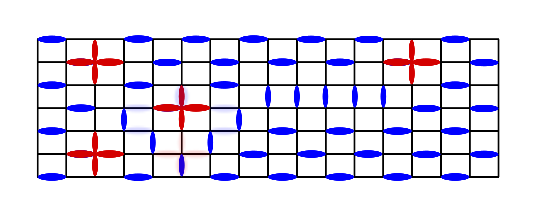
\includegraphics[width=8.5 cm]{ex_vert_mv_6}
    \caption{Step 6 in the vertical move example. Move the rightmost star of the new pair up.
    Rearrange the dimers around it to satisfy packing and conservation rules.\label{fig:ex_vert_mv_6}}
\end{figure}


% \bibliography{name_bib_file}

\end{document}
